\documentclass[aspectratio=169]{../latex_main/tntbeamer}  % you can pass all options of the beamer class, e.g., 'handout' or 'aspectratio=43'
\usepackage{dsfont}
\usepackage{bm}
\usepackage[english]{babel}
\usepackage[T1]{fontenc}
%\usepackage[utf8]{inputenc}
\usepackage{graphicx}
\graphicspath{ {./figures/} }
\usepackage{algorithm}
\usepackage[ruled,vlined,algo2e,linesnumbered]{algorithm2e}
\usepackage{hyperref}
\usepackage{booktabs}
\usepackage{mathtools}

\usepackage{amsmath,amssymb}

\DeclareMathOperator*{\argmax}{arg\,max}
\DeclareMathOperator*{\argmin}{arg\,min}

\usepackage{amsbsy}
\newcommand{\vect}[1]{\bm{#1}}
%\newcommand{\vect}[1]{\boldsymbol{#1}}

\usepackage{pgfplots}
\pgfplotsset{compat=1.16}
\usepackage{tikz}
\usetikzlibrary{trees} 
\usetikzlibrary{shapes.geometric}
\usetikzlibrary{positioning,shapes,shadows,arrows,calc,mindmap}
\usetikzlibrary{positioning,fadings,through}
\usetikzlibrary{decorations.pathreplacing}
\usetikzlibrary{intersections}
\pgfdeclarelayer{background}
\pgfdeclarelayer{foreground}
\pgfsetlayers{background,main,foreground}
\tikzstyle{activity}=[rectangle, draw=black, rounded corners, text centered, text width=8em]
\tikzstyle{data}=[rectangle, draw=black, text centered, text width=8em]
\tikzstyle{myarrow}=[->, thick, draw=black]

% Define the layers to draw the diagram
\pgfdeclarelayer{background}
\pgfdeclarelayer{foreground}
\pgfsetlayers{background,main,foreground}

% Requires XeLaTeX or LuaLaTeX
%\usepackage{unicode-math}

\usepackage{fontspec}
%\setsansfont{Arial}
\setsansfont{RotisSansSerifStd}[ 
Path=../latex_main/fonts/,
Extension = .otf,
UprightFont = *-Regular,  % or *-Light
BoldFont = *-ExtraBold,  % or *-Bold
ItalicFont = *-Italic
]
\setmonofont{Cascadia Mono}[
Scale=0.8
]

% scale factor adapted; mathrm font added (Benjamin Spitschan @TNT, 2021-06-01)
%\setmathfont[Scale=1.05]{Libertinus Math}
%\setmathrm[Scale=1.05]{Libertinus Math}

% other available math fonts are (not exhaustive)
% Latin Modern Math
% XITS Math
% Libertinus Math
% Asana Math
% Fira Math
% TeX Gyre Pagella Math
% TeX Gyre Bonum Math
% TeX Gyre Schola Math
% TeX Gyre Termes Math

% Literature References
\newcommand{\lit}[2]{\href{#2}{\footnotesize\color{black!60}[#1]}}

%%% Beamer Customization
%----------------------------------------------------------------------
% (Don't) Show sections in frame header. Options: 'sections', 'sections light', empty
\setbeamertemplate{headline}{empty}

% Add header logo for normal frames
\setheaderimage{
	% 
\includegraphics[height=\logoheight]{figures/TNT_darkv4.pdf}
	
\includegraphics[height=\logoheight]{../latex_main/figures/luh_logo_rgb_0_80_155.pdf}
	% 
\includegraphics[height=\logoheight]{figures/logo_tntluh.pdf}
}

% Header logo for title page
\settitleheaderimage{
	% 
\includegraphics[height=\logoheight]{figures/TNT_darkv4.pdf}
	
\includegraphics[height=\logoheight]{../latex_main/figures/luh_logo_rgb_0_80_155.pdf}
	% 
\includegraphics[height=\logoheight]{figures/logo_tntluh.pdf}
}

% Title page: tntdefault 
\setbeamertemplate{title page}[tntdefault]  % or luhstyle
% Add optional title image here
%\addtitlepageimagedefault{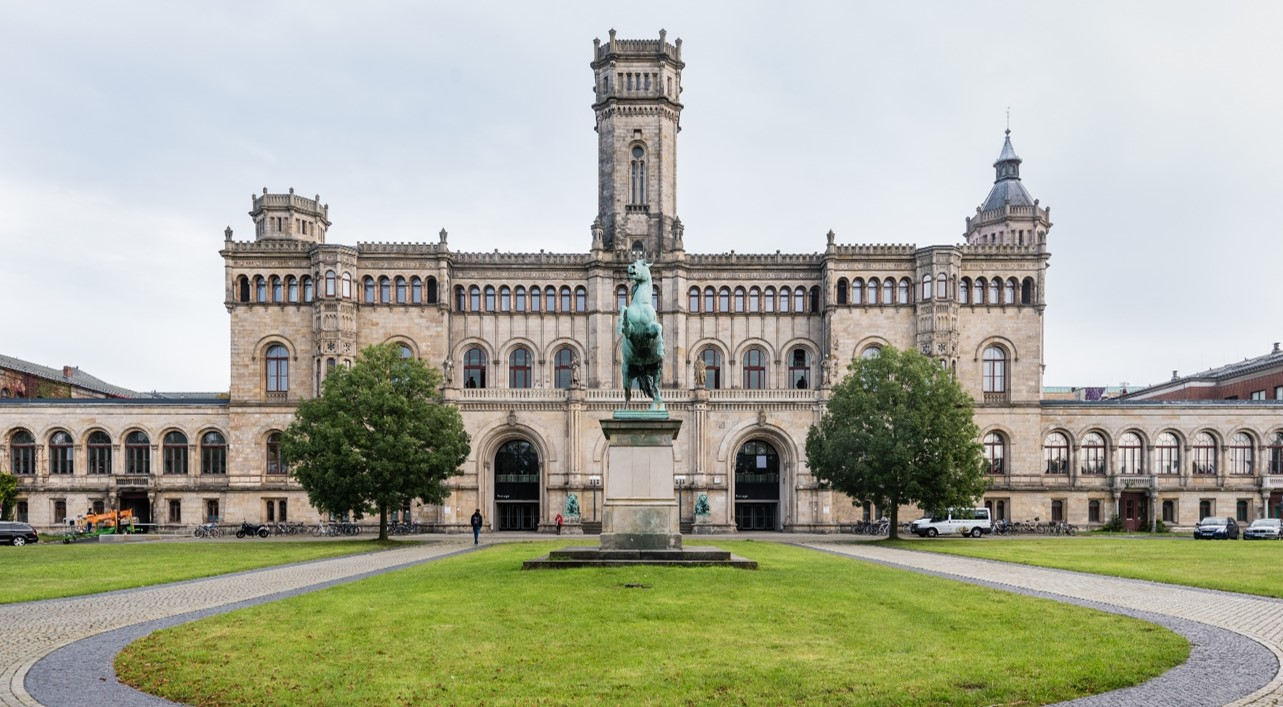
\includegraphics[width=0.65\textwidth]{figures/luh_default_presentation_title_image.jpg}}

% Title page: luhstyle
% \setbeamertemplate{title page}[luhstyle]
% % Add optional title image here
% \addtitlepageimage{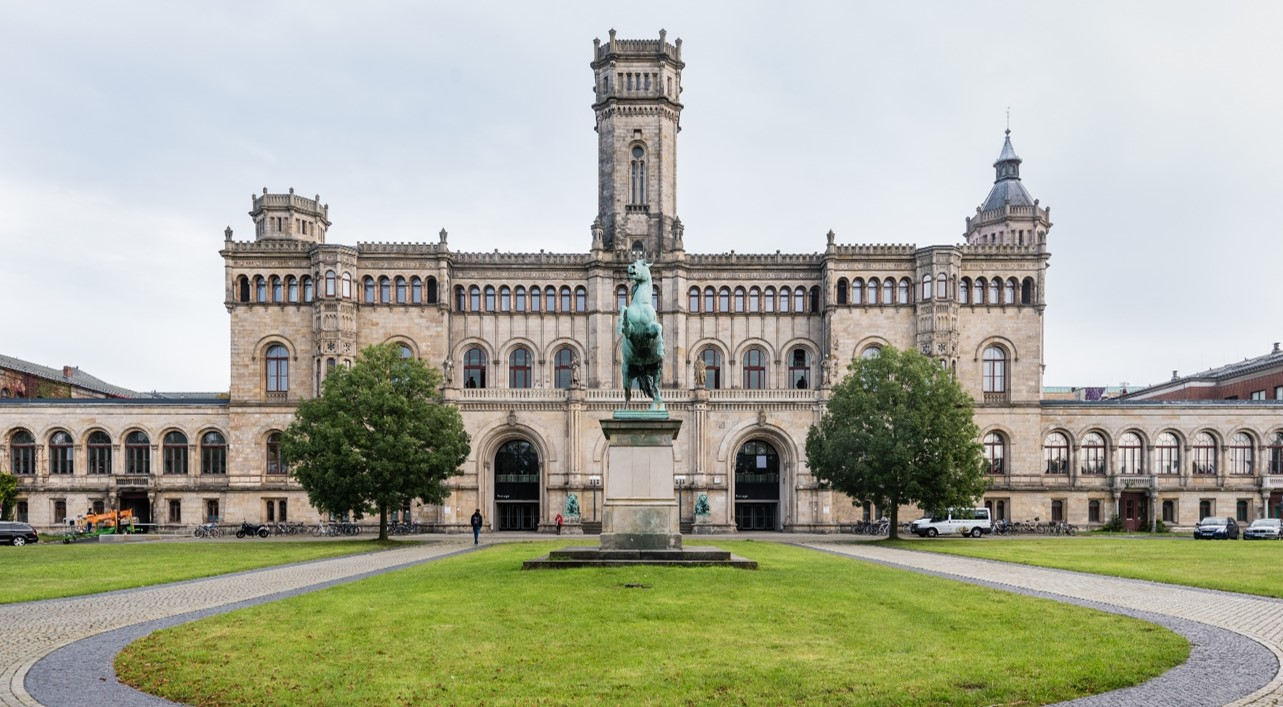
\includegraphics[width=0.75\textwidth]{figures/luh_default_presentation_title_image.jpg}}

\author[Abedjan \& Lindauer]{Ziawasch Abedjan \& Marius Lindauer\\[1em]
	
\includegraphics[height=\logoheight]{../latex_main/figures/luh_logo_rgb_0_80_155.pdf}\qquad
	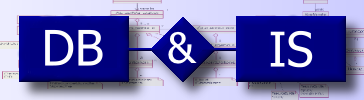
\includegraphics[height=\logoheight]{../latex_main/figures/DBIS_Kurzlogo.png}\qquad

\includegraphics[height=\logoheight]{../latex_main/figures/TNT_darkv4}\qquad

\includegraphics[height=\logoheight]{../latex_main/figures/L3S.jpg}	}
\date{Summer Term 2022; \hspace{0.5em} {
\includegraphics[height=1.5em]{../latex_main/figures/Cc-by-nc-sa_icon.svg.png}}; based on \href{https://ds100.org/fa21/}{[DS100]}
}


%%% Custom Packages
%----------------------------------------------------------------------
% Create dummy content
\usepackage{blindtext}

% Adds a frame with the current page layout. Just call \layout inside of a frame.
\usepackage{layout}


%%% Macros
%\renewcommand{\vec}[1]{\mathbf{#1}}
% \usepackage{bm}
%\let\vecb\bm

\title[Anomaly Detection]{DS: Learning}
\subtitle{Unsupervised Learning: Anomaly Detection}

\graphicspath{ {./figure/} }
%\institute{}


\begin{document}
	
    \maketitle
    
    \begin{frame}[c]{What is Anomaly Detection?}
        \begin{itemize}
            \item Unsupervised learning: Only input features $x$ are given, but no trainings labels
            \item Anomamly detection: Only data from a single class is given
            \begin{itemize}
                \item Typically, it is harder to collect data from the other class since anomalies should only happen rarely
            \end{itemize}
        \end{itemize} 

        \centering
        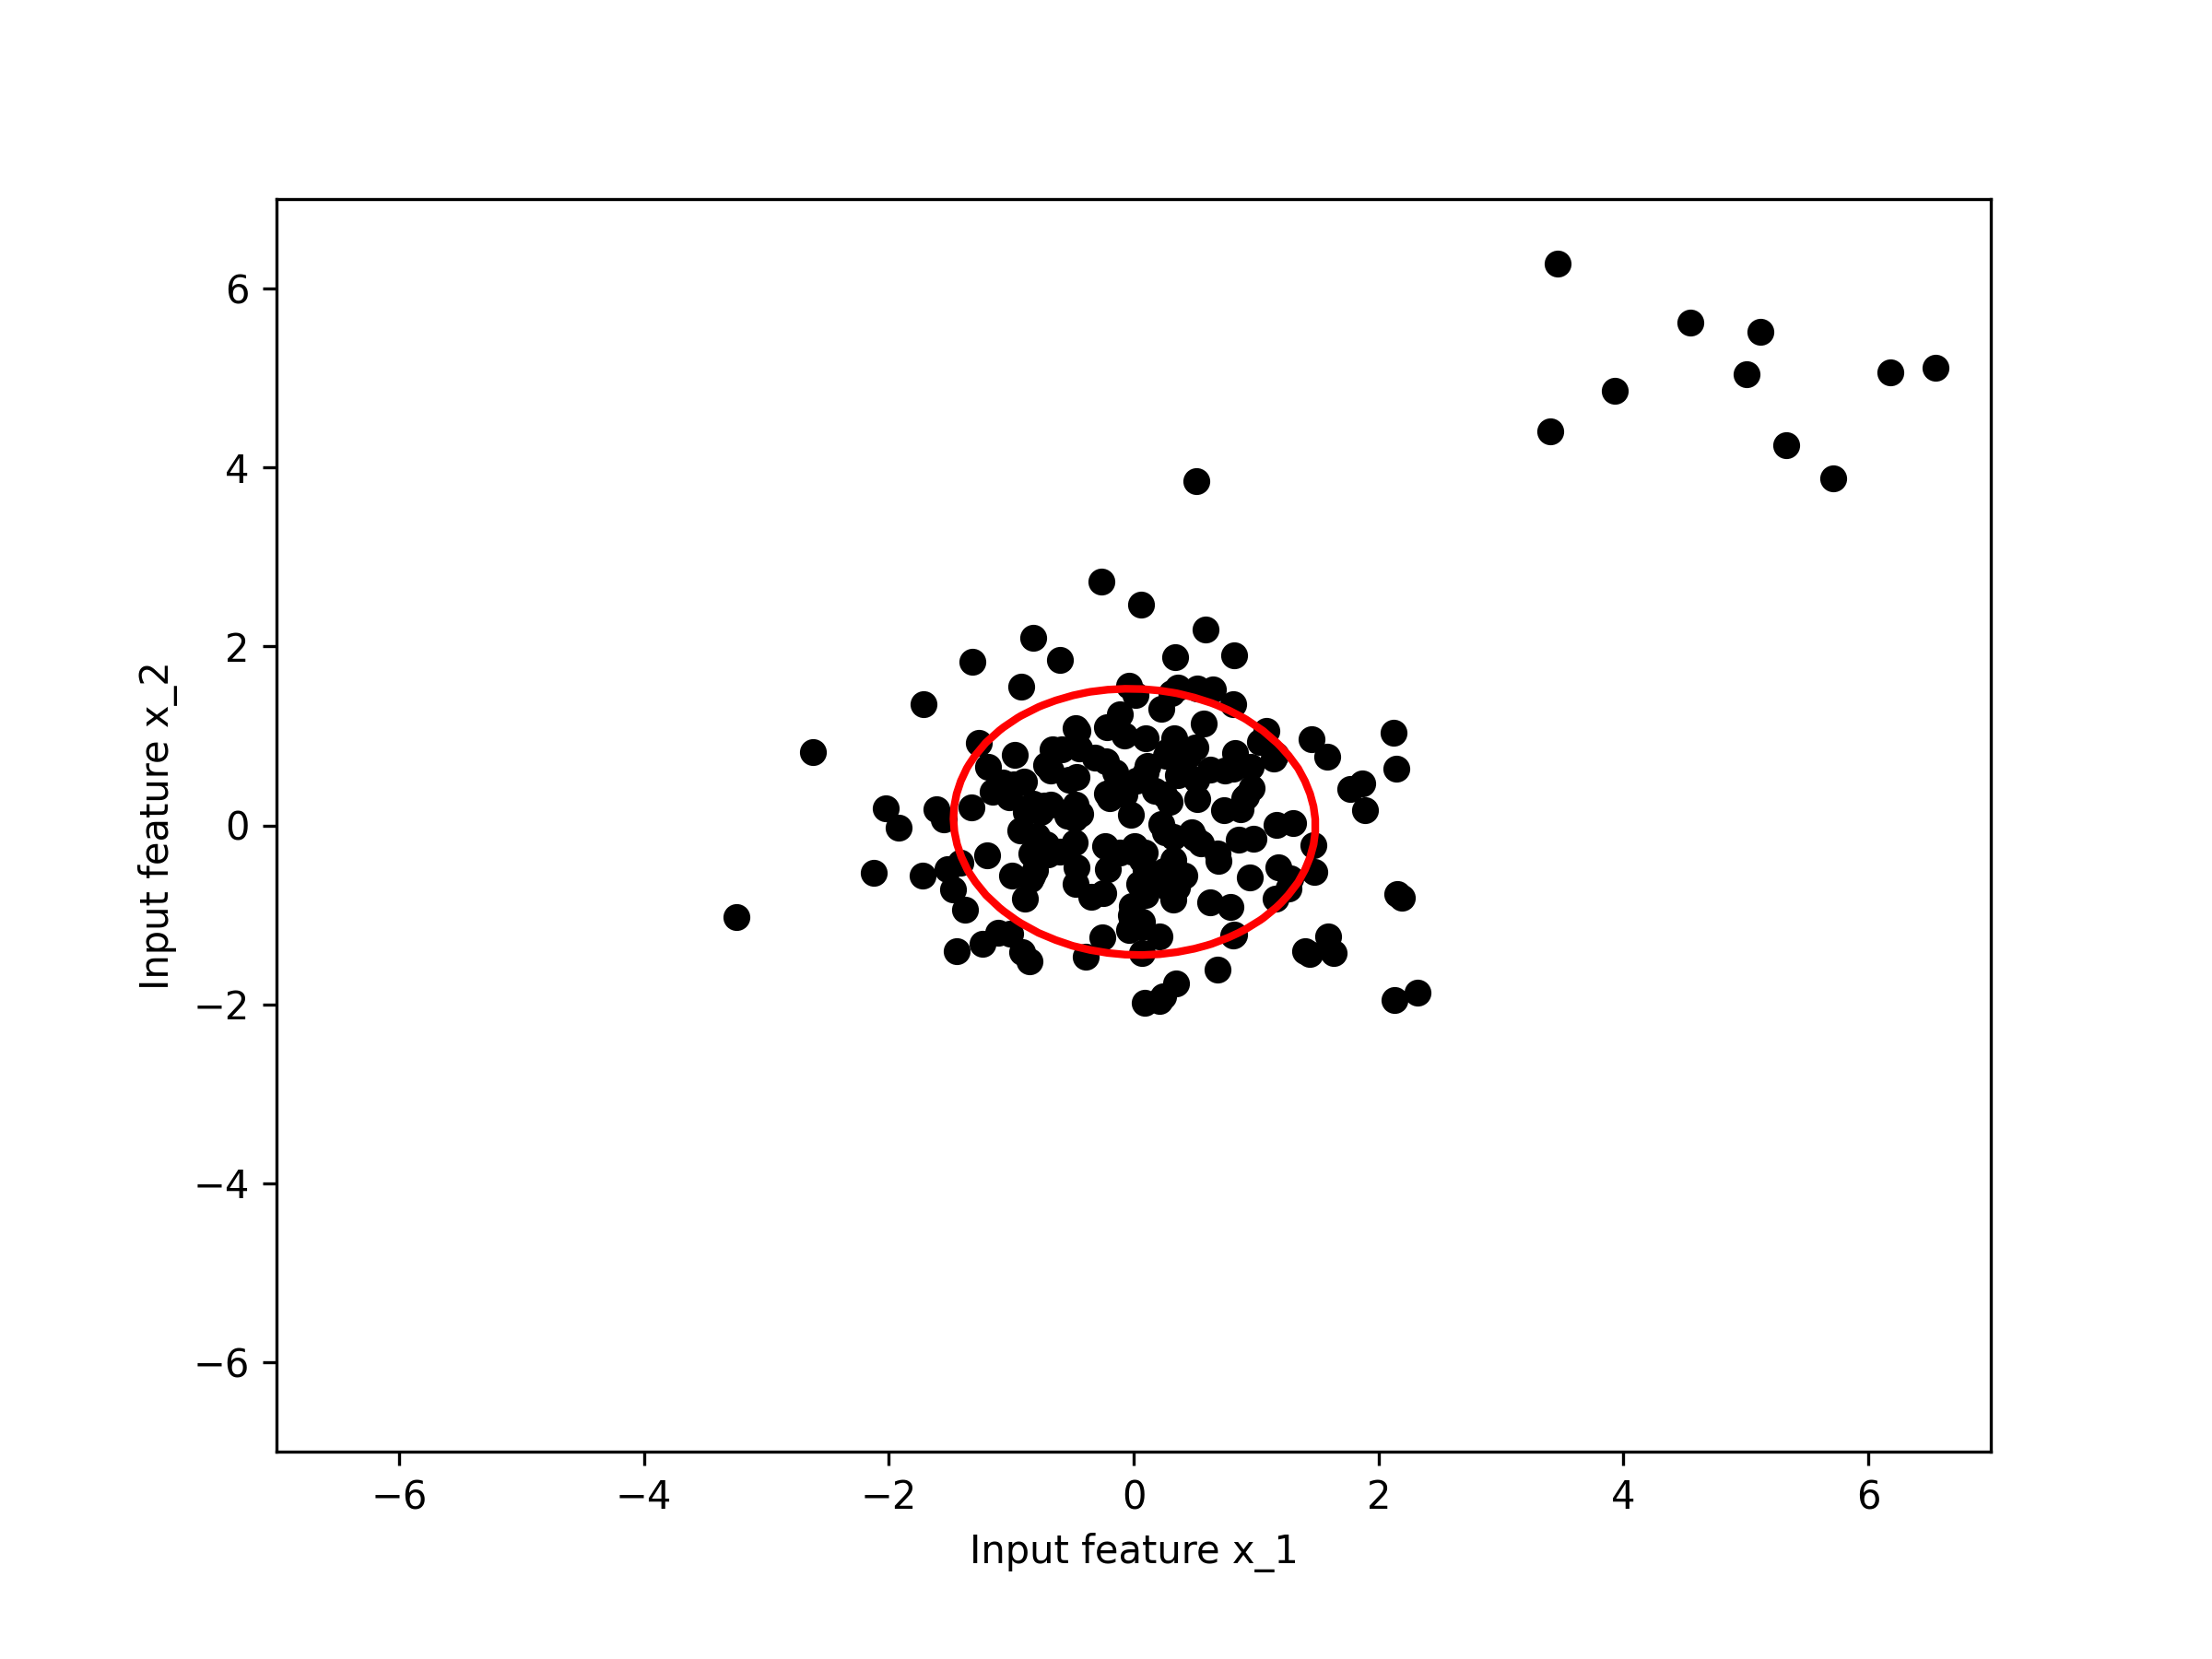
\includegraphics[width=0.5\textwidth]{figure/anomaly}

        % import numpy as np
        % import matplotlib.pyplot as plt
        % from sklearn.datasets import make_blobs
        % from sklearn.cluster import KMeans
        
        % # Generate some random training data with more pronounced clusters
        % X, y = make_blobs(n_samples=500, centers=4, random_state=42, cluster_std=1.5)
        
        % # Fit a clustering model
        % kmeans = KMeans(n_clusters=4, random_state=42)
        % y_pred = kmeans.fit_predict(X)
        
        % # Create a meshgrid to plot the decision boundaries
        % x_min, x_max = X[:, 0].min() - 1, X[:, 0].max() + 1
        % y_min, y_max = X[:, 1].min() - 1, X[:, 1].max() + 1
        % xx, yy = np.meshgrid(np.arange(x_min, x_max, 0.1), np.arange(y_min, y_max, 0.1))
        % Z = kmeans.predict(np.c_[xx.ravel(), yy.ravel()])
        
        % # Create a contour plot of the decision boundaries
        % Z = Z.reshape(xx.shape)
        % plt.contourf(xx, yy, Z, alpha=0.2)
        
        % # Create a scatter plot of the data
        % plt.scatter(X[:, 0], X[:, 1], c='black')
        
        % # Add axis labels and increase font size
        % plt.xlabel(r'Input feature $x_1$', fontsize=14)
        % plt.ylabel(r'Input feature $x_2$', fontsize=14)
        % plt.xticks(fontsize=12)
        % plt.yticks(fontsize=12)
        
        % plt.savefig('clustering.png', dpi=300)
        
        % # Show the plot
        % plt.show()

    \end{frame}

    

    \begin{frame}[c]{Anomaly Models (I)}
        \begin{description}
            \item[Density-Based Models] are based on the assumption that normal data points appear in high-density regions, while anomalies appear in low-density regions. Examples of density-based models include Gaussian Mixture Models (GMM), Local Outlier Factor (LOF), and Autoencoder-based methods.
            \pause
            \item[Distance-Based Models] detect anomalies based on their distance from the normal data points. Examples of distance-based models include k-Nearest Neighbors (k-NN) and Support Vector Data Description (SVDD).
            \pause
            \item[Reconstruction-Based Models] use reconstruction errors to identify anomalies. They learn the normal behavior of the system and flag anything that deviates significantly from it. Examples of reconstruction-based models include Principal Component Analysis (PCA), Isolation Forest, and Variational Autoencoder (VAE).
            \pause
            \item[Deep Learning Models] use deep neural networks to detect anomalies. Examples of deep learning models include Convolutional Autoencoder (CAE), Recurrent Neural Network (RNN), and Generative Adversarial Network (GAN).

        \end{description}

    \end{frame}


\end{document}